%%% License: Creative Commons Attribution Share Alike 4.0 (see https://creativecommons.org/licenses/by-sa/4.0/)


%%%%%%%%%%%%%%%%%%%%%%%%%%%%%%%%%%%%%%%%%

%----------------------------------------------------------------------------------------
%	PACKAGES AND OTHER DOCUMENT CONFIGURATIONS
%----------------------------------------------------------------------------------------

\documentclass[a4paper]{article}

\usepackage{amssymb}
\usepackage{enumitem}
\usepackage[usenames,dvipsnames]{color}
\usepackage{fancyhdr} % Required for custom headers
\usepackage{lastpage} % Required to determine the last page for the footer
\usepackage{extramarks} % Required for headers and footers
\usepackage[usenames,dvipsnames]{color} % Required for custom colors
\usepackage{graphicx} % Required to insert images
\usepackage{listings} % Required for insertion of code
\usepackage{courier} % Required for the courier font
\usepackage[table]{xcolor}
\usepackage{amsfonts,amsmath,amsthm,parskip,setspace,url}
\usepackage[section]{placeins}
\usepackage[a4paper]{geometry}
\usepackage[USenglish]{babel}
\usepackage[utf8]{inputenc}
\usepackage{tikz}


% Margins
\topmargin=-0.45in
\evensidemargin=0in
\oddsidemargin=0in
\textwidth=6.5in
\textheight=9.0in
\headsep=0.6in

\linespread{1.1} % Line spacing



%----------------------------------------------------------------------------------------
%   FORMATTING
%----------------------------------------------------------------------------------------
% Set up the header and footer
\pagestyle{fancy}
\lhead[c]{\textbf{{\color[rgb]{.5,0,0} K{\o}benhavns\\Universitet }}} % Top left header
\chead{\textbf{{\color[rgb]{.5,0,0} \Class }}\\ \hmwkTitle  } % Top center head
\rhead{\instructor \\ \theprofessor} % Top right header
\lfoot{\lastxmark} % Bottom left footer
\cfoot{} % Bottom center footer
\rfoot{Page\ \thepage\ of\ \protect\pageref{LastPage}} % Bottom right footer
\renewcommand\headrulewidth{0.4pt} % Size of the header rule
\renewcommand\footrulewidth{0.4pt} % Size of the footer rule


% Other formatting stuff
%\setlength\parindent{12pt}
\setlength{\parskip}{5 pt}
%\theoremstyle{definition} \newtheorem{ex}{\textbf{\Large{Exercise & #}\\}}
\usepackage{titlesec}
\titleformat{\section}[hang]{\normalfont\bfseries\Large}{Problem \thesection:}{0.5em}{}




%----------------------------------------------------------------------------------------
%	NAME AND CLASS SECTION
%----------------------------------------------------------------------------------------
\newcommand{\hmwkTitle}{Exercises after Lecture 14 (M7)} % Assignment title
\newcommand{\Class}{Mechanism Design} % Course/class
\newcommand{\instructor}{Fall 2020} % TA
\newcommand{\theprofessor}{Prof. Egor Starkov} % Professor




%----------------------------------------------------------------------------------------
%   SOLUTIONS
%----------------------------------------------------------------------------------------
\newif\ifsolutions
%\solutionstrue




\begin{document}

\begin{center}
		\LARGE\textbf{Exercises after Lecture 14 (M7):\\ Information design.}
\end{center}



\section{Two approaches to information design}
	
	Consider the following information design problem. There are two possible states, $\omega \in \{L,R\}$, the common prior belief that the state is $R$ is $\phi_0 = \mathbb{P}(\omega = R) = 1/2$. There is one player (receiver) and two actions $a \in \{u,d\}$ available to him. The receiver's payoffs as a function of state are given by the function $v_1(a,\omega)$, which is defined as
	\begin{center}
		\begin{tabular}{c | c | c |}
			$v_1(a,\omega)$ 		& $\omega = L$ 	& $\omega = R$ \\ \hline
			$a=u$	& $3$ 	& $0$	\\ \hline
			$a=d$	& $0$ 	& $1$	\\ \hline
		\end{tabular}
	\end{center}
	There is a designer who (before getting to observe $\omega$) designs an experiment that will send a message to the receiver, which may be informative about the true state $\omega$. The designer's payoff coincides with that of the receiver, with one exception: the designer receives a bribe of $4$ if action $a=d$ is chosen in state $\omega=L$. In other words, the designer's payoff function $\pi(a,\omega)$ is given by
	\begin{center}
		\begin{tabular}{c | c | c |}
			$v_0(a,\omega)$ 		& $\omega = L$ 	& $\omega = R$ \\ \hline
			$a=u$	& $3$ 	& $0$	\\ \hline
			$a=d$	& $4$ 	& $1$	\\ \hline
		\end{tabular}
	\end{center}
	
	\begin{enumerate}
		\item Derive the receiver's optimal action rule $\hat{a}(\phi)$, which maximizes his expected payoff, as a function of $\phi$, his posterior belief about the state after observing message $m$ generated by the experiment ($\phi = \mathbb{P} (\omega=R | m)$).
		\item Derive and plot the designer's payoff function $V_0(\phi) \equiv \mathbb{E}_{\phi(\omega)} \left[\pi (\hat{a}(\phi), \omega)\right]$ as a function of the receiver's posterior $\phi$.
		\item Derive and plot (on the same graph) the concave closure $V_0^* (\phi)$ of the receiver's payoff function $V_0(\phi)$.
		\item By looking at the plots of $V_0(\phi)$ and $V_0^* (\phi)$ and recalling that $\phi_0 = 1/2$, answer the following: what is the set of posteriors $\{\phi_1, \phi_2, ...\}$ induced by the optimal experiment (the one that maximizes the designer's expected payoff)? What is the designer's payoff from the optimal experiment?
		\item Use the ``correlated equilibria approach'' to find the optimal experiment. In particular, find a decision rule $\sigma: \{L,R\} \to \varDelta(\{u,d\})$ (so $\sigma(u|\omega)+\sigma(d|\omega)=1$ for any $\omega$) which maximizes the designer's expected payoff as given by
		\begin{equation*}
			v_0^* (\sigma) \equiv  \sum_{a,\omega} \pi(a,\omega) \sigma (a | \omega) \phi(\omega)
		\end{equation*}
		subject to the obedience constraint: for any $a,a' \in \{u,d\}$,
		\begin{align*}
			\sum_{\omega} v_1 (a, \omega) \sigma (a | \omega) \phi(\omega) 
			\geq \sum_{\omega} v_1 (a', \omega) \sigma (a | \omega) \phi(\omega) .
		\end{align*} 
	\end{enumerate}
	
	
\ifsolutions
\section*{Solution}

	\begin{enumerate}
		\item The receiver's expected utility of selecting $a=u$ is $\mathbb{E}_\phi v_1(u,\omega) = 3(1-\phi) + 0\phi$, while for $a=d$ it is $\mathbb{E}_\phi v_1(d,\omega) = 0(1-\phi) + 1\phi$. Taking the maximum of the two, the optimal action is
		\begin{align*}
			\hat{a}(\phi) = \begin{cases}
				u & \text{ if } \phi < 3/4;
				\\
				d & \text{ if } \phi \geq 3/4.
			\end{cases}
		\end{align*}
		Figure \ref{fig:twoappr_v1} plots utilities from both actions and the optimal action.
		
		\item Plugging the optimal action $\hat{a}(\omega)$ into the designer's payoff function and taking expectations w.r.t. $\phi(\omega)$ (the \emph{receiver's} posterior), we get
		\begin{align*}
			V_0(\phi) = \begin{cases}
				3-3\phi & \text{ if } \phi < 3/4;
				\\
				4-3\phi & \text{ if } \phi \geq 3/4.
			\end{cases}
		\end{align*}
		Note that we did indeed break the receiver's indifference in the designer's favor. This function is plotted in Figure \ref{fig:twoappr_v0}.
		\begin{figure}
			\parbox{0.5\linewidth}{
				\centering
				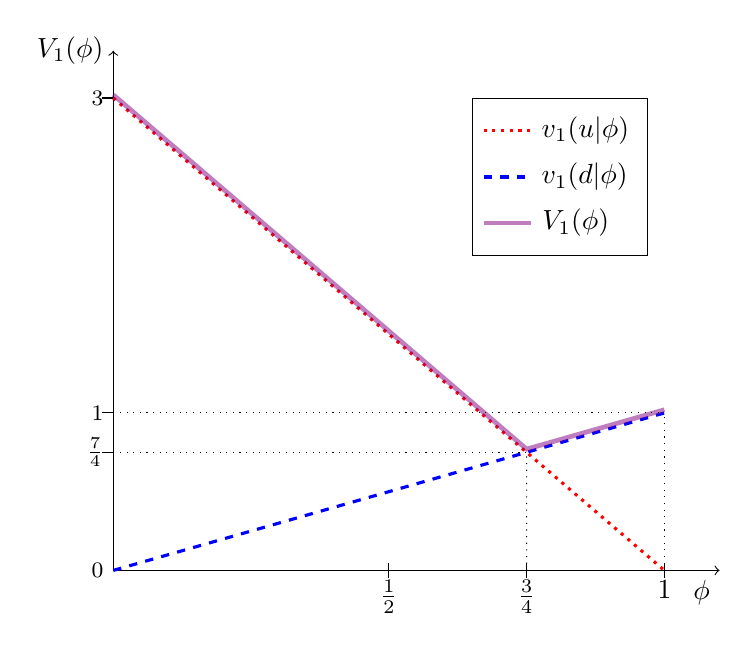
\begin{tikzpicture}[xscale=7,yscale=2]
					\draw[->] (0,0) -- (1.1,0) node[below left]{$\phi$};
					\draw[->] (0,0) -- (0,3.3) node[left]{$V_1(\phi)$};
					\draw (0,0) node[left]{\footnotesize $0$};
					
					% Plot
					\draw[line width=0.4mm, red, dotted] (0,3) -- (1,0);
					\draw[line width=0.4mm, blue, dashed] (0,0) -- (1,1);
					\draw[line width=0.6mm, violet, opacity=0.5] (0,3.02) -- (0.75,0.77) -- (1,1.02);
					
					% Ticks
					% x axis
					\draw (0.5,0) coordinate(q1) node[below]{$\frac{1}{2}$};
					\draw (q1) ++(0,-0.05) -- ++(0,0.1);
					
					\draw (0.75,0) coordinate(q2) node[below]{$\frac{3}{4}$};
					\draw (q2) ++(0,-0.05) -- ++(0,0.1);
					\draw[dotted] (q2) -- (0.75,0.75);
					
					\draw (1,0) coordinate(q3) node[below]{$1$};
					\draw (q3) ++(0,-0.05) -- ++(0,0.1);
					\draw[dotted] (1,0) -- (1,1);
					
					% y axis
					\draw (0,1) coordinate(u1) node[left]{\footnotesize $1$};
					\draw (u1) ++(-0.02,0) -- ++(0.02,0);
					\draw[dotted] (u1) -- ++(1,0);
					
					\draw (0,0.75) coordinate(u2) node[left]{\footnotesize $\frac{7}{4}$};
					\draw (u2) ++(-0.02,0) -- ++(0.02,0);
					\draw[dotted] (u2) -- ++(0.75,0);
					
					\draw (0,3) coordinate(u3) node[left]{\footnotesize $3$};
					\draw (u3) ++(-0.02,0) -- ++(0.02,0);
					
					%Legend
					\matrix [draw, fill=white, below right] at (0.65,3) {
						\draw [line width=0.4mm, red, dotted] ++(-0.3,0) -- ++(0.6,0) node[black,right] {$v_1(u|\phi)$}; \\
						\draw [line width=0.4mm, blue, dashed] ++(-0.3,0) -- ++(0.6,0) node[black,right] {$v_1(d|\phi)$}; \\
						\draw [line width=0.6mm, violet, opacity=0.5] ++(-0.3,0) -- ++(0.6,0) node[black,right,opacity=1] {$V_1(\phi)$}; \\
					};
				\end{tikzpicture}
				\caption{$V_1(\phi)$}
				\label{fig:twoappr_v1}
			}
			\parbox{0.5\linewidth}{
				\centering
				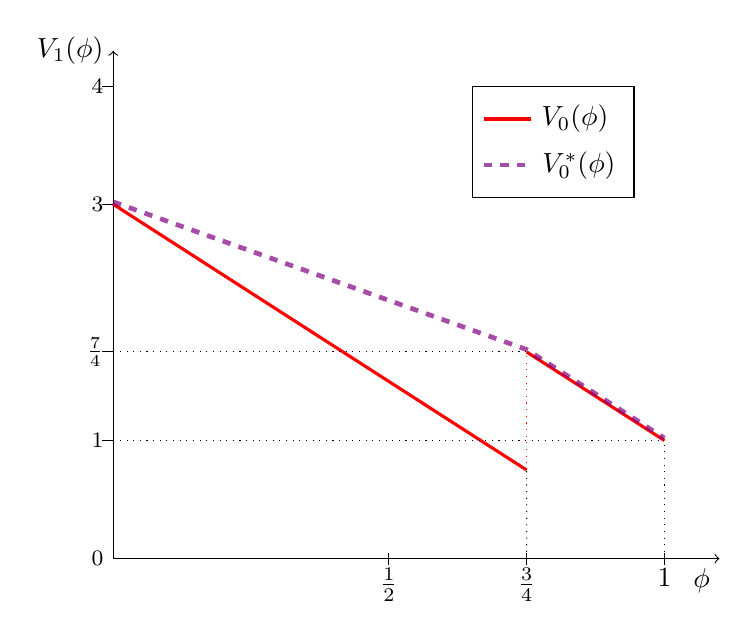
\begin{tikzpicture}[xscale=7,yscale=1.5,
						piline/.style={line width=0.4mm, red}
					]
					\draw[->] (0,0) -- (1.1,0) node[below left]{$\phi$};
					\draw[->] (0,0) -- (0,4.3) node[left]{$V_1(\phi)$};
					\draw (0,0) node[left]{\footnotesize $0$};
					
					% Plot
					\draw[piline] (0,3) -- (0.75,0.75);
					\draw[red,dotted] (0.75,0.75) -- (0.75,1.75);
					\draw[piline] (0.75,1.75) -- (1,1);
					\draw[line width=0.6mm, violet, opacity=0.7, dashed] (0,3.02) -- (0.75,1.77) -- (1,1.02);
					
					% Ticks
					% x axis
					\draw (0.5,0) coordinate(q1) node[below]{$\frac{1}{2}$};
					\draw (q1) ++(0,-0.05) -- ++(0,0.1);
					
					\draw (0.75,0) coordinate(q2) node[below]{$\frac{3}{4}$};
					\draw (q2) ++(0,-0.05) -- ++(0,0.1);
					\draw[dotted] (q2) -- (0.75,0.75);
					
					\draw (1,0) coordinate(q3) node[below]{$1$};
					\draw (q3) ++(0,-0.05) -- ++(0,0.1);
					\draw[dotted] (1,0) -- (1,1);
					
					% y axis
					\draw (0,1) coordinate(u1) node[left]{\footnotesize $1$};
					\draw (u1) ++(-0.02,0) -- ++(0.02,0);
					\draw[dotted] (u1) -- ++(1,0);
					
					\draw (0,1.75) coordinate(u2) node[left]{\footnotesize $\frac{7}{4}$};
					\draw (u2) ++(-0.02,0) -- ++(0.02,0);
					\draw[dotted] (u2) -- ++(0.75,0);
					
					\draw (0,3) coordinate(u3) node[left]{\footnotesize $3$};
					\draw (u3) ++(-0.02,0) -- ++(0.02,0);
					
					\draw (0,4) coordinate(u4) node[left]{\footnotesize $4$};
					\draw (u4) ++(-0.02,0) -- ++(0.02,0);
					
					%Legend
					\matrix [draw, fill=white, below right] at (0.65,4) {
						\draw [piline] ++(-0.3,0) -- ++(0.6,0) node[black,right] {$V_0(\phi)$}; \\
						\draw [line width=0.6mm, violet, opacity=0.7, dashed] ++(-0.3,0) -- ++(0.6,0) node[black,right,opacity=1] {$V_0^*(\phi)$}; \\
					};
				\end{tikzpicture}
				\caption{$V_0(\phi)$ and $V_0^*(\phi)$}
				\label{fig:twoappr_v0}
			}
		\end{figure}
	
		\item See Figure \ref{fig:twoappr_v0}.
		
		\item The set of optimal posteriors is given the set of $\phi$ that are such that $V_0^*(\phi) = V_0(\phi)$. Starting from $\phi_0=1/2$, we see from Figure \ref{fig:twoappr_v0} that the two closest such posteriors are $\phi=0$ and $\phi=3/4$. 
		
		Designer's optimal payoff is given by
		\begin{align*}
		V_0^*(\phi) = \begin{cases}
			3-\frac{5}{3}\phi & \text{ if } \phi < 3/4;
			\\
			4-3\phi & \text{ if } \phi \geq 3/4.
		\end{cases}
		\end{align*}
		(since it is a piecewise-linear function passing through points $(\phi,V_0^*) = \{(0,3);(3/4,7/4);(1,1)\}$). Plugging in the prior $\phi_0$, we get that the designer's expected payoff given this prior is $3-5/6 = 13/6$.
		
		\item The designer's problem is:
		\begin{align*}
			\max_\sigma & \left\{ \left(3\sigma(u|L) + 4 \sigma(d|L)\right)\frac{1}{2} + \left(0\sigma(u|R) + 1 \sigma(d|R)\right)\frac{1}{2} \right\}
			\\
			\text{s.t. } 
			& 3 \sigma(u|L)\frac{1}{2} + 0 \sigma(u|R)\frac{1}{2} \geq 0 \sigma(u|L)\frac{1}{2} + 1 \sigma(u|R)\frac{1}{2}
			\\
			& 0 \sigma(d|L)\frac{1}{2} + 1 \sigma(d|R)\frac{1}{2} \geq 3 \sigma(d|L)\frac{1}{2} + 0 \sigma(d|R)\frac{1}{2}
			\\
			& \sigma(u|L) + \sigma(d|L) = 1
			\\
			& \sigma(u|R) + \sigma(d|R) = 1
		\end{align*}
		(plus the implicit constraints $\sigma(a|\omega)\in[0,1]$ for all $a,\omega$).
		After scaling the objective function and the first two constraints up by a factor of 2 (to get rid of irrelevant $\frac{1}{2}$s), omitting the zeroes, and then also expressing $\sigma(d|\omega) = 1-\sigma(u|\omega)$ for $\omega \in \{L,R\}$ from the two last constraints, the problem reduces to:
		\begin{align*}
			\max_{\sigma(u|L),\sigma(u|R)} & \left\{ 3\sigma(u|L) + 4 (1-\sigma(u|L)) + (1-\sigma(u|R)) \right\}
			\\
			\text{s.t. } 
			& 3 \sigma(u|L) \geq \sigma(u|R)
			\\
			& 1-\sigma(u|R)\geq 3 (1-\sigma(u|L))
		\end{align*}
		or, equivalently,
		\begin{align*}
			\max_{\sigma(u|L),\sigma(u|R)} & \left\{ 5 - \sigma(u|L) - \sigma(d|R) \right\}
			\\
			\text{s.t. } 
			& \sigma(u|R) \leq 3 \sigma(u|L)
			\\
			& \sigma(u|R)\leq 3\sigma(u|L)-2
		\end{align*}
		So we want to select $\sigma(u|R)$ and $\sigma(u|L)$ as low as possible. It is immediate that $\sigma(u|R)=0$ is optimal. The first obedience constraint is then satisfied automatically (again, given the implied constraint $\sigma(u|L) \geq 0$). From the second constraint we get $\sigma(u|L) \geq 2/3$, thus in the optimum $\sigma(u|L) = 2/3$.
		
		In the end, the solution is:
		\begin{align*}
			\sigma(u|L) &= 2/3	&	\sigma(d|L) &= 1-\sigma(u|L) = 1/3;
			\\
			\sigma(u|R) &= 0	&	\sigma(d|R) &= 1-\sigma(u|R) = 1.
		\end{align*}
	\end{enumerate}
	
\fi




\section{Final-2019, p4}
	
	A consumer is choosing between two Samsung smartphones: the new Galaxy Fold, which costs $p_F = \$ 2000$, and the older Galaxy S10, which costs $p_S = \$1000$. The consumer does not know which of the two is right for her, and she is very afraid of making the wrong choice. 
	
	Formally, from the consumer's point of view, one of the two states is possible: $\omega \in \{F,S\}$. Her expected utility from buying phone $a \in \{F,S\}$ is given by
	\begin{equation*}
		v_1(a|\phi) = \mathbb{E}_\omega \left[ w(a,\omega) \mid \phi \right] - p_a,
	\end{equation*}
	where $\phi$ denotes the probability that the consumer assigns to state being $\omega = F$, and the state-dependent valuations $w(a,\omega)$ are given by
	\begin{center}
		\begin{tabular}{c | c | c |}
			$w(a,\omega)$ 		& $\omega = F$ 	& $\omega = S$ \\ \hline
			$a=F$ (buy Fold)	& $3000$ 	& $0$	\\ \hline
			$a=S$ (buy S10)		& $0$ 	& $1500$	\\ \hline
		\end{tabular}
	\end{center}
	The consumer always has the option (denoted as $a = \varnothing$) to walk away from the purchase, which yields utility zero in both states.
	
	The seller can procure the phones at zero cost, hence his profit $v_0(a)$ is given by
	\begin{equation*}
		v_0(a) = 
		\begin{cases}
			p_F & \text{ if } a=F; \\
			p_S & \text{ if } a=S; \\
			0 & \text{ if } a=\varnothing.
		\end{cases}
	\end{equation*}
	
	\begin{enumerate}
		\item %(4pts) 
		Describe the consumer's optimal choice rule $a(\phi)$ for any given belief $\phi = \mathbb{P}(\omega=F)$.
		\item %(4pts) 
		Write down the consumer's expected utility $V_1(\phi) = \max_a v_1(a|\phi)$ from following this optimal choice rule $a(\phi)$. 
		\item %(4pts) 
		Write down the company's profit $V_0(\phi)$ from the consumer following her optimal choice rule $a(\phi)$.
	\end{enumerate}
	
	Suppose that the consumer's prior is $\phi_0 = \frac{1}{2}$. The seller decides to engage in Bayesian Persuasion: he designs a quiz that, when passed by the consumer, will tell her which phone is likely better for her. Formally, a quiz is an experiment $\mu = \left\{ (\tau_1, \phi_1), (\tau_2, \phi_2), ... \right\}$, which moves the consumer's belief to $\phi_k$ with probability $\tau_k$. Naturally, it must be that $\sum_k \tau_k = 1$ and $\sum_k \tau_k \phi_k = \phi_0$. Note that posteriors $\phi_k$ need not be in $\{0,1\}$: the quiz may induce any posterior belief $\phi_k \in [0,1]$.
	\begin{enumerate}[resume]
		\item %(13pts) 
		Find the quiz/experiment $\mu$ that maximizes the seller's expected profit. \\%Find the expected profit generated by this experiment.
		\emph{Hint: drawing a graph of $V_0(\phi)$ may help you.}
	\end{enumerate}
	
	
\ifsolutions
\subsection*{Solution}
	
	\begin{figure}
		\parbox{0.5\linewidth}{
			\centering
			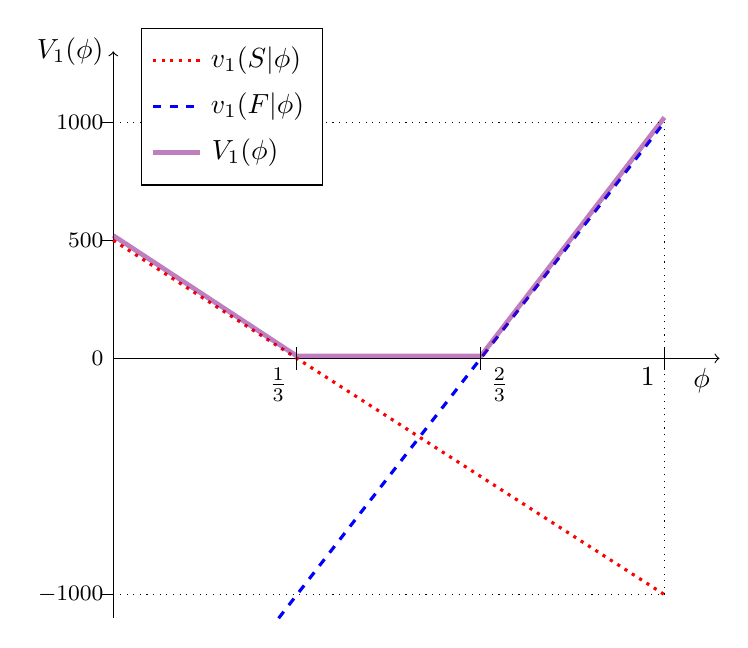
\begin{tikzpicture}[xscale=7,yscale=3]
				\draw[->] (0,0) -- (1.1,0) node[below left]{$\phi$};
				\draw[->] (0,-1.1) -- (0,1.3) node[left]{$V_1(\phi)$};
				\draw (0,0) node[left]{\footnotesize $0$};
				
				% Plot
				\draw[line width=0.4mm, red, dotted] (0,0.5) -- (1,-1);
				\draw[line width=0.4mm, blue, dashed] (0.3,-1.1) -- (1,1);
				\draw[line width=0.6mm, violet, opacity=0.5] (0,0.52) -- (0.333,0.01) -- (0.667,0.01) -- (1,1.02);
				
				% Ticks
				% x axis
				\draw (0.333,0) coordinate(q1) node[below left]{$\frac{1}{3}$};
				\draw (q1) ++(0,-0.05) -- ++(0,0.1);
				
				\draw (0.667,0) coordinate(q2) node[below right]{$\frac{2}{3}$};
				\draw (q2) ++(0,-0.05) -- ++(0,0.1);
				
				\draw (1,0) coordinate(q3) node[below left]{$1$};
				\draw (q3) ++(0,-0.05) -- ++(0,0.1);
				\draw[dotted] (1,-1) -- (1,1);
				
				% y axis
				\draw (0,0.5) coordinate(u1) node[left]{\footnotesize $500$};
				\draw (u1) ++(-0.02,0) -- ++(0.02,0);
				
				\draw (0,1) coordinate(u2) node[left]{\footnotesize $1000$};
				\draw (u2) ++(-0.02,0) -- ++(0.02,0);
				\draw[dotted] (u2) -- ++(1,0);
				
				\draw (0,-1) coordinate(u3) node[left]{\footnotesize $-1000$};
				\draw (u3) ++(-0.02,0) -- ++(0.02,0);
				\draw[dotted] (u3) -- ++(1,0);
				
				%Legend
				\matrix [draw, fill=white, below right] at (0.05,1.4) {
					\draw [line width=0.4mm, red, dotted] ++(-0.3,0) -- ++(0.6,0) node[black,right] {$v_1(S|\phi)$}; \\
					\draw [line width=0.4mm, blue, dashed] ++(-0.3,0) -- ++(0.6,0) node[black,right] {$v_1(F|\phi)$}; \\
					\draw [line width=0.6mm, violet, opacity=0.5] ++(-0.3,0) -- ++(0.6,0) node[black,right,opacity=1] {$V_1(\phi)$}; \\
				};
			\end{tikzpicture}
			\caption{$V_1(\phi)$}
			\label{fig:U}
		}
		\parbox{0.5\linewidth}{
			\centering
			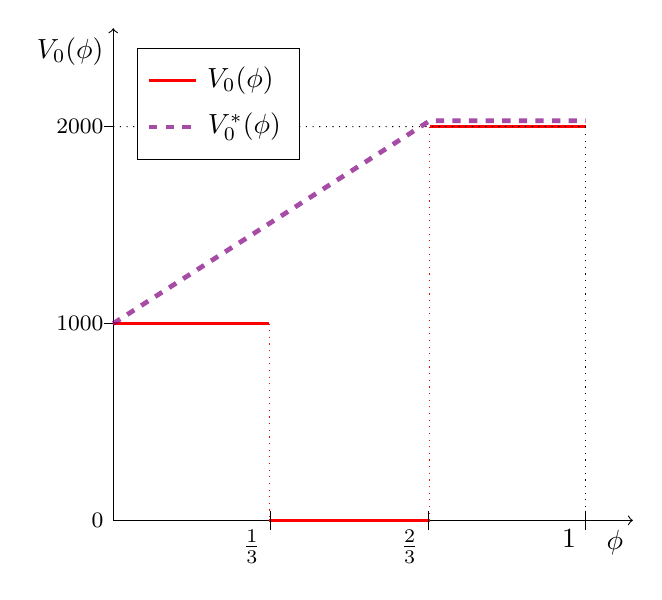
\begin{tikzpicture}[xscale=6,yscale=2.5,
				piline/.style={line width=0.4mm, red}
				]
				\draw[->] (0,0) -- (1.1,0) node[below left]{$\phi$};
				\draw[->] (0,0) -- (0,2.5) node[below left]{$V_0(\phi)$};
				\draw (0,0) node[left]{\footnotesize $0$};
				
				% Plot
				% Pi
				\draw[piline] (0,1) -- (0.33,1);
				\draw[red,dotted] (0.33,1) -- (0.33,0);
				\draw[piline] (0.33,0) -- (0.67,0);
				\draw[red,dotted] (0.67,0) -- (0.67,2);
				\draw[piline] (0.67,2) -- (1,2);
				
				\draw[line width=0.6mm, violet, opacity=0.7, dashed] (0,1) -- (0.67,2.03) -- (1,2.03);
				
				% Ticks
				% x axis
				\draw (0.333,0) coordinate(q1) node[below left]{$\frac{1}{3}$};
				\draw (q1) ++(0,-0.05) -- ++(0,0.1);
				
				\draw (0.667,0) coordinate(q2) node[below left]{$\frac{2}{3}$};
				\draw (q2) ++(0,-0.05) -- ++(0,0.1);
				
				\draw (1,0) coordinate(q3) node[below left]{$1$};
				\draw (q3) ++(0,-0.05) -- ++(0,0.1);
				\draw[dotted] (1,0) -- (1,2);
				
				% y axis
				\draw (0,1) coordinate(u1) node[left]{\footnotesize $1000$};
				\draw (u1) ++(-0.02,0) -- ++(0.02,0);
				
				\draw (0,2) coordinate(u2) node[left]{\footnotesize $2000$};
				\draw (u2) ++(-0.02,0) -- ++(0.02,0);
				\draw[dotted] (u2) -- (1,2);
				
				%Legend
				\matrix [draw, fill=white, below right] at (0.05,2.4) {
					\draw [piline] ++(-0.3,0) -- ++(0.6,0) node[black,right] {$V_0(\phi)$}; \\
					\draw [line width=0.6mm, violet, opacity=0.7, dashed] ++(-0.3,0) -- ++(0.6,0) node[black,right,opacity=1] {$V_0^*(\phi)$}; \\
				};
			\end{tikzpicture}
			\caption{$V_0(\phi)$ and $V_0^*(\phi)$}
			\label{fig:profit}
		}
	\end{figure}
	
	\begin{enumerate}
		\item The consumer's utilities from the three options are given by:
		\begin{align*}
			v_1(F|\phi) &= \phi \cdot 3000 + (1-\phi) \cdot 0 - 2000 \\
			v_1(S|\phi) &= \phi \cdot 0 + (1-\phi) \cdot 1500 - 1000 \\
			v_1(\varnothing|\phi) &= 0
		\end{align*}
		The three are depicted in Figure \ref{fig:U}.
		Taking the maximum of the three for a given $\phi$ yields the optimal choice rule
		\begin{equation*}
			a(\phi) = 
			\begin{cases}
				F & \text{ if } \phi \geq \frac{2}{3}; \\
				\varnothing & \text{ if } \phi \in \left[ \frac{1}{3}, \frac{2}{3} \right]; \\
				S & \text{ if } \phi \leq \frac{1}{3}.
			\end{cases}
		\end{equation*}
		\item From the previous answer, we get
		\begin{equation*}
			V_1(\phi) = 1000 \cdot 
			\begin{cases}
				3\phi - 2 & \text{ if } \phi \geq \frac{2}{3}; \\
				0 & \text{ if } \phi \in \left[ \frac{1}{3}, \frac{2}{3} \right]; \\
				0.5 - 1.5\phi & \text{ if } \phi \leq \frac{1}{3}.
			\end{cases}
		\end{equation*}
		\item From (1), we have
		\begin{equation*}
			V_0(\phi) = 1000 \cdot 
			\begin{cases}
				2 & \text{ if } \phi \geq \frac{2}{3}; \\
				0 & \text{ if } \phi \in \left[ \frac{1}{3}, \frac{2}{3} \right]; \\
				1 & \text{ if } \phi \leq \frac{1}{3}.
			\end{cases}
		\end{equation*}
		\item As suggested by the hint, look at the graph of $V_0(\phi)$ depicted in Figure \ref{fig:profit}.
		The profit $V_0^*(\phi)$ that the seller can achieve under the optimal Bayesian Persuasion mechanism is given by the smallest concave envelope of $V_0(\phi)$. You can see from the Figure that $V_0^*(\phi)$ coincides with $V_0(\phi)$ for $\phi \in NP \equiv \{0\} \cup [2/3,1]$ -- if the consumer's prior belonged to this set then no persuasion mechanism could increase the seller's profit. For any remaining prior (which includes our case, $\phi_0=1/2$), the optimal persuasion mechanism splits the prior between two closest points in $NP$. In case of prior $\phi_0 = 1/2$, the optimal persuasion mechanism prescribes posteriors $\phi_1 = 0$ and $\phi_2 = 2/3$. The probabilities of these posteriors can then be computed from the consistency requirement (a.k.a. law of total probability):
		\begin{align*}
			\tau_1 \cdot \phi_1 + \tau_2 \cdot \phi_2 &= \phi_0
			\\
			\Leftrightarrow \tau_1 \cdot 0 + \tau_2 \cdot \frac{2}{3} &= \frac{1}{2}
		\end{align*}
		and the requirement $\tau_1 + \tau_2 = 1$. The two together yield $(\tau_1,\tau_2) = (1/4, 3/4)$. Hence the optimal experiment $\mu$ induces posterior $\phi_1 = 0$ with probability $\tau_1 = 1/4$ and posterior $\phi_2 = 2/3$ with probability $\tau_2 = 3/4$.
		
		Note: graph in Figure \ref{fig:profit_wrong} is \textbf{not} considered correct (since the resulting $V_0^*(\phi)$ is not concave).
	\end{enumerate}
	
	\begin{figure}
		\centering
		\begin{tikzpicture}[xscale=6,yscale=2.5,
			piline/.style={line width=0.4mm, red}
			]
			\draw[->] (0,0) -- (1.1,0) node[below left]{$\phi$};
			\draw[->] (0,0) -- (0,2.5) node[below left]{$V_0(\phi)$};
			\draw (0,0) node[left]{\footnotesize $0$};
			
			% Plot
			% Pi
			\draw[piline] (0,1) -- (0.33,1);
			\draw[red,dotted] (0.33,1) -- (0.33,0);
			\draw[piline] (0.33,0) -- (0.67,0);
			\draw[red,dotted] (0.67,0) -- (0.67,2);
			\draw[piline] (0.67,2) -- (1,2);
			
			\draw[line width=0.6mm, violet, opacity=0.7, dashed] (0,1.03) -- (0.33,1.03) -- (0.67,2.03) -- (1,2.03);
			
			% Ticks
			% x axis
			\draw (0.333,0) coordinate(q1) node[below left]{$\frac{1}{3}$};
			\draw (q1) ++(0,-0.05) -- ++(0,0.1);
			
			\draw (0.667,0) coordinate(q2) node[below left]{$\frac{2}{3}$};
			\draw (q2) ++(0,-0.05) -- ++(0,0.1);
			
			\draw (1,0) coordinate(q3) node[below left]{$1$};
			\draw (q3) ++(0,-0.05) -- ++(0,0.1);
			\draw[dotted] (1,0) -- (1,2);
			
			%Legend
			\matrix [draw, fill=white, below right] at (0.05,2.4) {
				\draw [piline] ++(-0.3,0) -- ++(0.6,0) node[black,right] {$V_0(\phi)$}; \\
				\draw [line width=0.6mm, violet, opacity=0.7, dashed] ++(-0.3,0) -- ++(0.6,0) node[black,right,opacity=1] {$V_0^*(\phi)$}; \\
			};
		\end{tikzpicture}
		\caption{Incorrect $V_0^*(\phi)$}
		\label{fig:profit_wrong}
	\end{figure}
\fi

\end{document}
